% --------------------------------------
% Document Class
% --------------------------------------
\documentclass[a4paper,11pt]{article}
% --------------------------------------



% --------------------------------------
% Use Package
% --------------------------------------


\usepackage[francais]{babel}
%\usepackage{ucs}
\usepackage[utf8]{inputenc}
\usepackage[T1]{fontenc}

\usepackage{makeidx}
\usepackage{color}
\usepackage{graphicx}
\usepackage{float}
\usepackage[hidelinks]{hyperref} 
\usepackage{geometry}
%\usepackage{lastpage}
%\usepackage{marginnote}
\usepackage{fancyhdr}
%\usepackage{titlesec}
%\usepackage{framed}
\usepackage{amsmath}
\usepackage{empheq}
\usepackage{array}
\usepackage{multicol}
%\usepackage{adjustbox}

% insert code
\usepackage{listings}

% define our color
\usepackage{xcolor}

% code color
\definecolor{ligthyellow}{RGB}{250,247,220}
\definecolor{darkblue}{RGB}{5,10,85}
\definecolor{ligthblue}{RGB}{1,147,128}
\definecolor{darkgreen}{RGB}{8,120,51}
\definecolor{darkred}{RGB}{160,0,0}

% other color
\definecolor{ivi}{RGB}{141,107,185}


\lstset{
    language=Scilab,
    captionpos=b,
    extendedchars=true,
    frame=lines,
    numbers=left,
    numberstyle=\tiny,
    numbersep=5pt,
    keepspaces=true,
    breaklines=true,
    showspaces=false,
    showstringspaces=false,
    breakatwhitespace=false,
    stepnumber=1,
    showtabs=false,
    tabsize=3,
    basicstyle=\small\ttfamily,
    backgroundcolor=\color{ligthyellow},
    keywordstyle=\color{ligthblue},
    morekeywords={include, printf, uchar},
    identifierstyle=\color{darkblue},
    commentstyle=\color{darkgreen},
    stringstyle=\color{darkred},
}


% --------------------------------------



% --------------------------------------
% Page setting
% --------------------------------------
%\pagestyle{empty}
\setlength{\headheight}{15pt}

\setcounter{secnumdepth}{3}
\setcounter{tocdepth}{2}

\makeatletter
\@addtoreset{chapter}{part}
\makeatother 

\hypersetup{         % parametrage des hyperliens
  colorlinks=true,      % colorise les liens
  breaklinks=true,      % permet les retours à la ligne pour les liens trop longs
  urlcolor= blue,       % couleur des hyperliens
  linkcolor= black,     % couleur des liens internes aux documents (index, figures, tableaux, equations,...)
  citecolor= green      % couleur des liens vers les references bibliographiques
}

% --------------------------------------

% --------------------------------------
% Information
% --------------------------------------
\title{Compte-rendu TP2 TI : Projection perspective}
\author{Elliot VANEGUE et Gaëtan DEFLANDRE}
% --------------------------------------

\definecolor{myColor}{rgb}{0.5, 0.1, 0.75}

% --------------------------------------
% Begin content
% --------------------------------------
\begin{document}

% Set language to english
  \selectlanguage{francais}

  % Start the page counting
  \pagenumbering{arabic}

  \maketitle
  
  \mbox{}
  \newpage
  \clearpage
  
  \section*{Introduction}
  Lors de ce TP, nous allons voir les différentes étapes permettant de passer d'un
  modèle 3D à un modèle 2D. Pour cela nous avons besoin de calculer les matrices 
  extrinsèque et intrinsèque qui vont nous aider à déterminer les coordonnées des points
  d'une image 3D dans sa représentation 2D.
  
  \section{Modèles d'objets 3D et affichage 2D}
  Dans un premier temps nous allons faire varier les paramètres présent dans l'exemple fournit
  dans le cadre de ce TP afin d'observer la réaction de l'objet.\\
  
  \begin{figure}[H]
    \center
    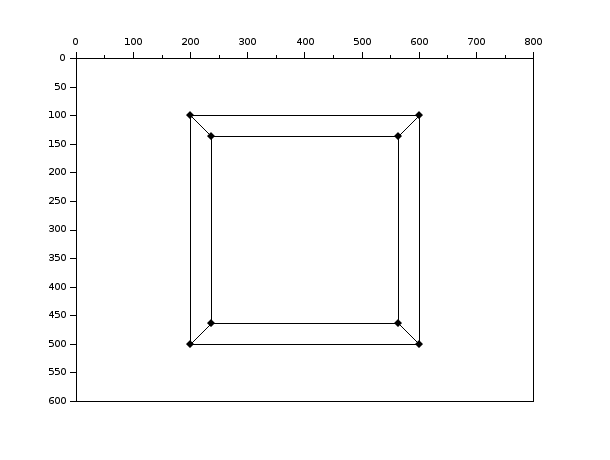
\includegraphics[width=10cm]{Projection1.png}
    \caption{Image du cube avec la matrice de projection de base}
  \end{figure}

  
  Au départ, nous avons une matrice de projection qui vaut : 
  $\begin{pmatrix}
   -360 & 0 & 80 & 400 \\
   0 & -360 & 60 & 300 \\
   0 & 0 & 0.2 & 1
  \end{pmatrix}$
  Nous avons constater que si nous modifions les valeurs -360, nous interagissions sur la largeur
  et la hauteur du carré. Lorsque nous modifions les valeurs 80 ou 60, la caméra fesait une rotation
  autour du carré. Et si nous modifions les valeurs 400 ou 300, la caméra translatait.\\
  
  \begin{figure}[H]
    \center
    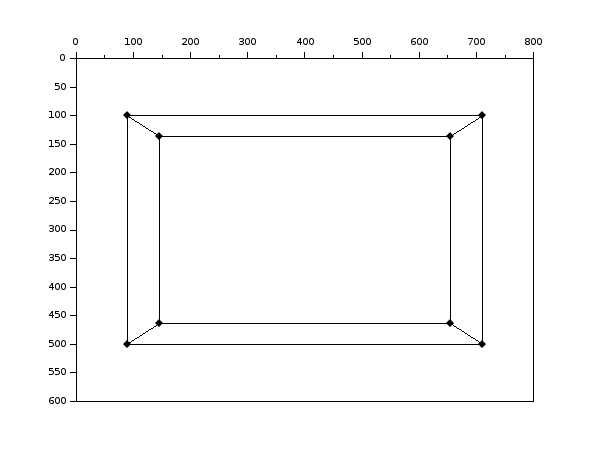
\includegraphics[width=5cm]{ProjectionTaille.png}
    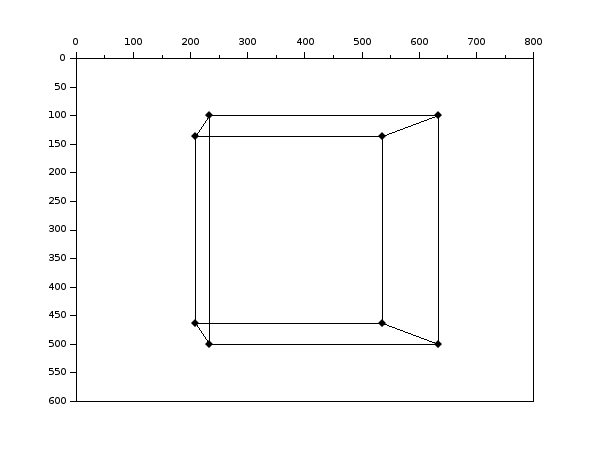
\includegraphics[width=5cm]{ProjectionRotation.png}
    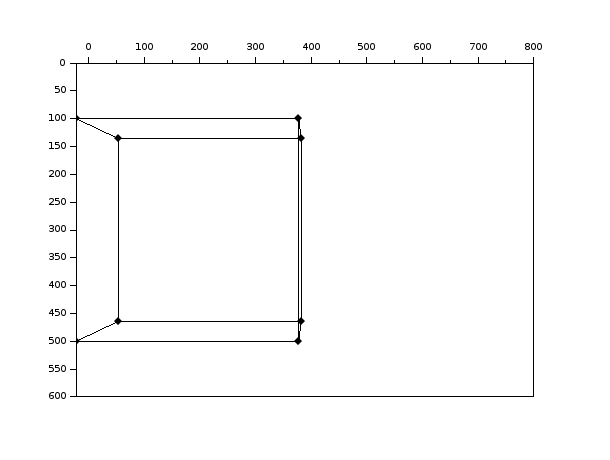
\includegraphics[width=5cm]{ProjectionTranslation.png}
    \caption{Image du cube avec modification des valeur de la matrice de projection}
  \end{figure}
  
  Nous avons ensuite modifié ces paramètres sur une grille 2D. Nous remarquons que 
  les transformations cités précédemment sont également valide pour cette forme 
  excepté la rotation. Etant donné que cette forme n'est pas 3D, il n'existe pas 
  de segment reliant deux points de coordonnées différentes dans l'axe x et donc aucune
  modification de distance entre deux points n'est possible sur cette axe.

  \section{Matrice extrinsèque}
  
  Nous allons maintenant chercher à calculer la matrice extrinsèque. Cette matrice prend en compte
  des paramètres qui dépendent de la position de la caméra dans l'espace de travail, comme la rotation
  ou la translation effectué par la caméra. Pour calculer cette matrice, nous l'avons décomposé en 
  plusieurs sous matrice que nous devrons multiplier. Voici les matrices composant la matrice extrinsèque :\\
  
  \begin{itemize}
   \item matrice de rotation x : 
   $\begin{pmatrix}
     1 & 0 & 0\\
     0 & cos(theta) & -sin(theta)\\
     0 & sin(theta) & cos(theta)
    \end{pmatrix}$
    
   \item matrice de rotation y : 
   $\begin{pmatrix}
     cos(theta) & 0 & sin(theta)\\
     0 & 1 & 0\\
     -sin(theta) & 0 & cos(theta)
    \end{pmatrix}$
    
   \item matrice de rotation z : 
   $\begin{pmatrix}
     cos(theta) & -sin(theta) & 0\\
     sin(theta) & cos(theta) & 0\\
     0 & 0 & 1
    \end{pmatrix}$
    
   \item matrice de translation : 
   $\begin{pmatrix}
     x\\
     y\\
     z
    \end{pmatrix}$

  \end{itemize}
  
  Une fois ces matrices définit, nous les multiplions afin d'obtenir la matrice
  extrinsèque qui à la forme suivante :\\
  \begin{center}
    $\begin{pmatrix}
      R_{x/x} & R_{x/y} & R_{x/z} & t_{x}\\
      R_{y/x} & R_{y/y} & R_{y/z} & t_{y}\\
      R_{z/x} & R_{z/y} & R_{z/z} & t_{z}\\
      0 & 0 & 0 & 1
      \end{pmatrix}$
  \end{center}

  Nous avons ensuite calculer les matrices extrinsèques de deux exemples du TP.
  \begin{itemize}
   \item E1 : Cette exemple place la caméra en dessous du cube. Pour cela il suffit
   d'effectué une translation de la caméra sur l'axe z. Ce qui nous donne la matrice
   extrinsèque 
    $\begin{pmatrix}
      0\\
      0\\
      5
      \end{pmatrix}$
   \item E2 : Dans cette exemple la caméra se positionne à 5m sur la diagonale principale.
   La caméra regarde donc un des coins supérieur du cube. Pour cela il faut que la caméra 
   fasse une rotation sur y de 45\degre pour que la caméra regarde une des arêtes du cube. Puis,
   il faut faire une rotation de ...%TODO effectué le calcul de l'angle
   sur l'axe z. Et enfin, effectué une translation de 5m sur la caméra sur l'axe x.
   %TODO noté la matrice résultante
  \end{itemize}
  
  \section{Matrice intrinsèque}
  
  Nous allons maintenant calculer la matrice intrinsèque qui dépend de paramètres propre à la caméra comme
  sa distance focale, les facteurs d'agrandissement de l'image... 
  \section{Projection et affichage des objets}
  
  
  \section*{Conclusion}
  
    
\end{document}